\documentclass{article}
\usepackage[utf8]{inputenc}
\usepackage[hidelinks]{hyperref}
\usepackage{color}
\usepackage{graphics}
\usepackage{graphicx}
\usepackage[spanish]{babel}

\title{Matemáticas Computacionales \\ Practica 3: Métodos Numéricos}
\author{1860560 Rangel Delgado Jesus Angel}
\date{26 de Marzo del 2021}

\begin{document}

\maketitle

\section{Introducción}
En esta practica se estudiara el método de bisección, un tema que sera aplicado con códigos en R y con algunos ejemplos, además se estudiara la teoría sobre dicho tema.

\section{Método de bisección}
\subsection{¿Qué es?}
Este es uno de los métodos más sencillos y de fácil
intuición, para resolver ecuaciones en una variable. Se
basa en el Teorema de los Valores Intermedios, el cual
establece que toda función continua f en un intervalo
cerrado [a,b] 
\begin{equation}
    ( f \in C[a,b] )
\end{equation}
toma todos los valores que
se hallan entre f(a) y f(b). Esto es, que todo valor entre
f (a) y f (b) es la imagen de al menos un valor en el
intervalo [a,b].

\subsection{¿En que consiste?}
El método consiste en lo siguiente: Supongamos que en el intervalo [a,b] hay un cero de f . Calculamos el punto
medio m = (a +b)/2 del intervalo [a,b]. A continuación calculamos f (m). En caso de que f (m) sea igual a cero,
ya hemos encontrado la solución buscada. En caso de que no lo sea, verificamos si f (m) tiene signo opuesto al
de f (a). Se redefine el intervalo [a,b] como [a,m] o [m,b] según se haya determinado en cuál de estos intervalos
ocurre un cambio de signo. A este nuevo intervalo se le aplica el mismo procedimiento y así, sucesivamente, iremos
encerrando la solución en un intervalo cada vez más pequeño, hasta alcanzar la precisión deseada.

\newpage
\begin{figure}[h]
    \centering
    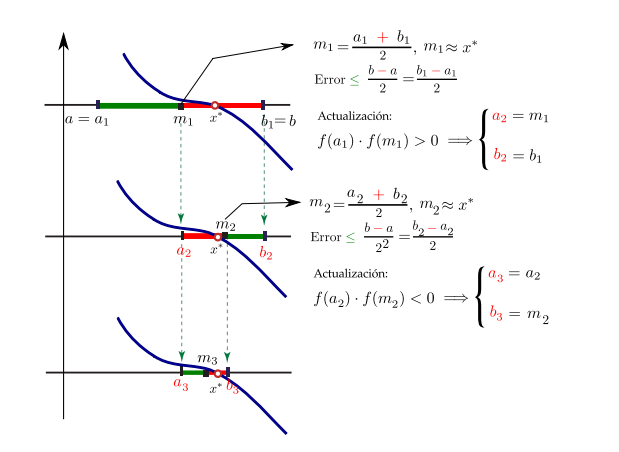
\includegraphics[width=12cm, height=8cm]{ejemplo1.PNG}
    \caption{Ilustración de lo explicado anteriormente}
    \label{fig:mesh1}
\end{figure}

\subsection{Estimación del error}
El error exacto en el k-ésimo paso en \[|m_{k} - x^{*}|\].
Geométricamente se puede ver esto que esto es menos que la mitad del intervalo \[|a_{k} - b_{k}|\] es decir:
\newline

\begin{equation}
    |m_{k} - x^{*}| \leq \frac{b_{k}-a_{k}}{2}= \frac{b-a}{2^{k}}
\end{equation}

\newpage
\section{Código en R}
Para trabajar estos métodos en esta practica se asigno un código cuya funcionalidad es la de gráficar y obtener valores aplicando el método de bisección en base a una ecuación o un intervalo dado.
\begin{figure}[h]
    \centering
    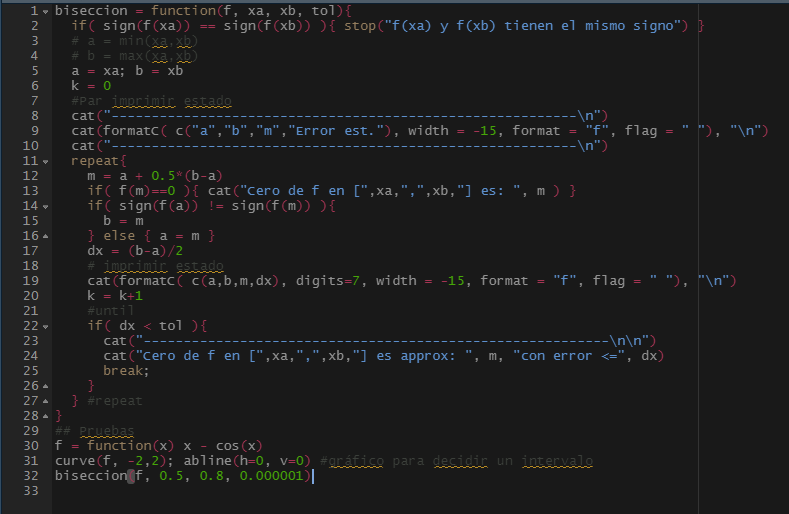
\includegraphics[width=12cm, height=8cm]{codigobase.PNG}
    \caption{Código para aplicar el método de bisección}
    \label{fig:mesh2}
\end{figure}

\subsection{Ejercicio 1}
En el código Resolver 
\begin{equation}
    x^{3}= 0
\end{equation}
Usando bisección en el intervalo [-0,2, 0.1].
\newpage

\begin{figure}[h]
    \centering
    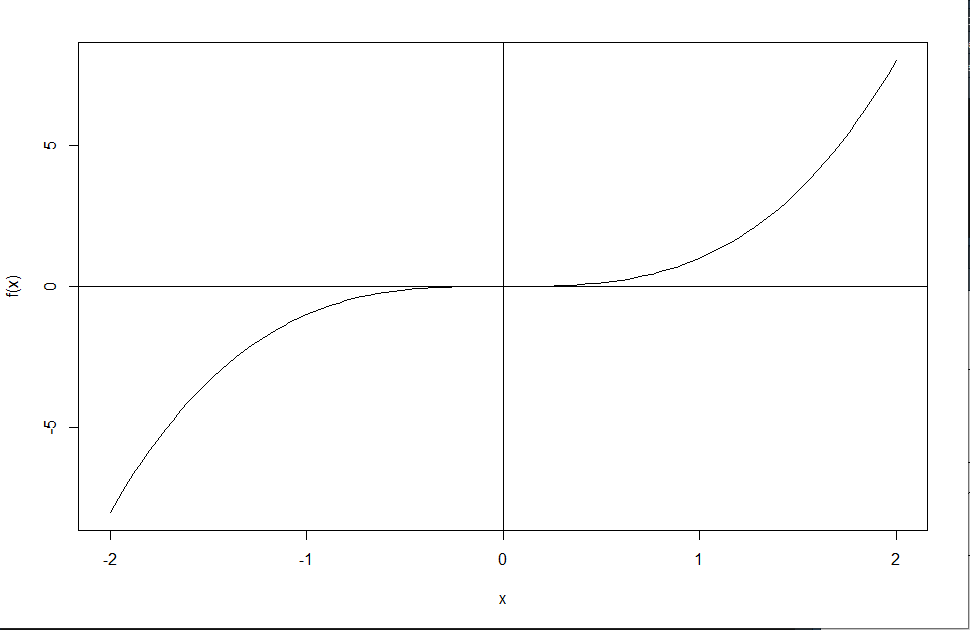
\includegraphics[width=10cm, height=5cm]{grafica1.PNG}
    \caption{Gráfica Solución}
    \label{fig:mesh3}
\end{figure}

\begin{figure}[h]
    \centering
    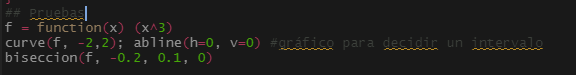
\includegraphics[width=10cm, height=2cm]{codigografica1.PNG}
    \caption{Código para la gráfica}
    \label{fig:mesh4}
\end{figure}

\newpage

\begin{figure}[h]
    \centering
    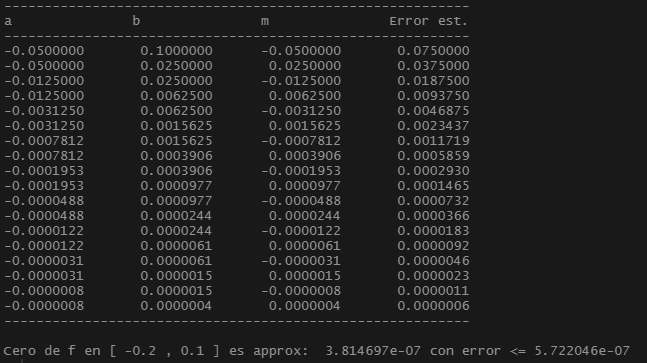
\includegraphics[width=12cm, height=8cm]{Tabla1.PNG}
    \caption{Tabla generada al ejecutar el código}
    \label{fig:mesh5}
\end{figure}

\subsection{Ejercicio 2}
En el código Resolver 
\begin{equation}
    f= x^{5}-100x^{4}+3995x^{3}-79700x^{2}+794004x-3160075
\end{equation}
Usando bisección en el intervalo [-0.2, 0.1].

\newpage

\begin{figure}[h]
    \centering
    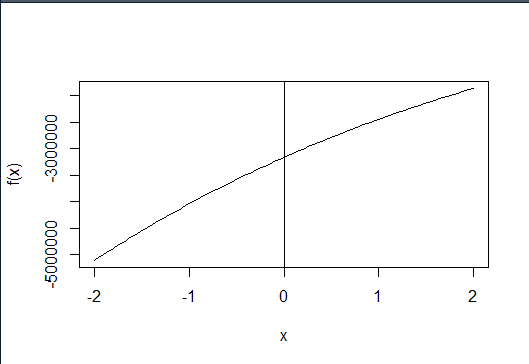
\includegraphics[width=10cm, height=5cm]{grafica2.PNG}
    \caption{Gráfica Solución}
    \label{fig:mesh6}
\end{figure}

\begin{figure}[h]
    \centering
    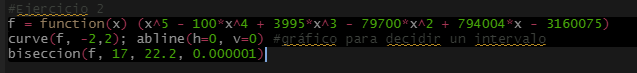
\includegraphics[width=10cm, height=2cm]{codigografica2.PNG}
    \caption{Código para la gráfica}
    \label{fig:mesh7}
\end{figure}

\newpage

\begin{figure}[h]
    \centering
    \includegraphics[width=12cm, height=8cm]{Tabla2.PNG}
    \caption{Tabla generada al ejecutar el código}
    \label{fig:mesh8}
\end{figure}

\subsection{Ejercicio 3}
En el código Resolver 
\begin{equation}
    x^{3}-2x-5=0
\end{equation}
para este ejercicio se uso el intervalo [2, 9]
\newpage

\begin{figure}[h]
    \centering
    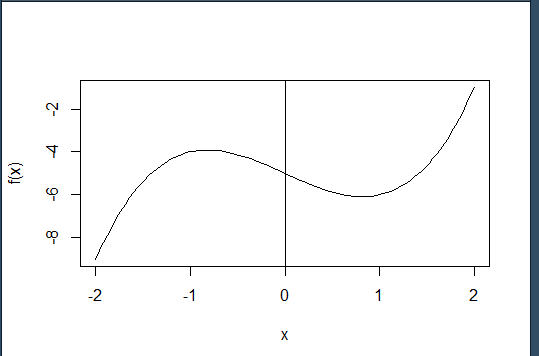
\includegraphics[width=10cm, height=5cm]{grafica3.PNG}
    \caption{Gráfica Solución}
    \label{fig:mesh9}
\end{figure}

\begin{figure}[h]
    \centering
    \includegraphics[width=10cm, height=2cm]{codigografica3.PNG}
    \caption{Código para la gráfica}
    \label{fig:mesh10}
\end{figure}

\newpage

\begin{figure}[h]
    \centering
    \includegraphics[width=12cm, height=8cm]{Tabla3.PNG}
    \caption{Tabla generada al ejecutar el código}
    \label{fig:mesh11}
\end{figure}

\begin{thebibliography}{0}
  \bibitem{Introducción a los métodos Numéricos, 2015} Mora F. Walter,Introducción a los métodos Numéricos , 2015
  \bibitem{Jesus Rangel, Repositorio de GitHub}Jesus Rangel, repositorio de GitHub\textcolor{blue}{\url{https://github.com/JesusRangel07/MatematicasComputacionales}}\href{https://github.com/JesusRangel07/MatematicasComputacionales}{\textcolor{blue}{Repositorio de Github}}
\end{thebibliography}

\end{document}
